\documentclass[10pt]{article}
\usepackage[utf8]{inputenc}
\usepackage{lipsum}
\usepackage{titlesec}
\usepackage{graphicx}
\usepackage{geometry}
\usepackage{setspace}
\usepackage{url}
\usepackage[breaklinks]{hyperref}

% Set up the page margins
\geometry{a4paper, margin=1in}

% Set up the depth for the Table of Contents
% Up to subsubsection is numbered
\setcounter{tocdepth}{3}
% Up to subsubsection is included in the Table of Contents
\setcounter{secnumdepth}{3}

% Adjust abstract and content formatting
\renewcommand{\abstractname}{\large\textbf{Abstract}}
\titleformat{\section}{\normalfont\large\bfseries}{\thesection}{1em}{}
\titleformat{\subsection}{\normalfont\normalsize\bfseries}{\thesubsection}{1em}{}

% Adjust document spacing
\onehalfspacing

\begin{document}
\begin{figure}
    \centering
    
\includegraphics[width=1.0\linewidth]{logo.png}
    
    \label{fig:enter-label}
\end{figure}

\title{
\vspace{\baselineskip}
SOEN 6841 - SOFTWARE PROJECT MANAGEMENT\\

\vspace{\baselineskip}
Prof. Pankaj Kamthan
\vspace{\baselineskip}
\\ Topic Analysis and Synthesis \\
\vspace{\baselineskip}

"DO LESS, LEAD MORE" \\
\vspace{\baselineskip}
GitHub Repository : \href{https://github.com/Gouthamsusarla/TAS-SOEN-6841}{Click Here!}

\vspace{\baselineskip}
}

\author{Goutham Susarla - 40232232}

\date{November 30, 2022}

\maketitle

\newpage


\begin{abstract}
\begin{normalsize}
\vspace{\baselineskip}
The topic "Do Less, Lead More" explores the pivotal transition faced by engineering managers as they ascend in their roles, often grappling with the challenge of balancing an expanding array of responsibilities. From the initial shift to management, managing multiple teams, to handling growth spurts in a startup, leaders frequently encounter a tipping point where the conventional approach of attempting to do everything becomes counterproductive. The narrative delves into the common pitfalls of overcommitment and the adverse effects on decision-making, sleep patterns, and overall team dynamics.

\vspace{\baselineskip}

Highlighting the manager's dilemma, the discourse emphasizes a crucial managerial superpower — the intentional decision to not do certain tasks. The narrative unfolds with strategic decision-making processes, guiding managers on adapting to new leadership roles and strategically choosing priorities through the "bad news test." It stresses the significance of task delegation, particularly when leading multiple teams.

\vspace{\baselineskip}

The concept of transparent leadership takes centre stage, advocating for open communication about priorities, responsibilities, and strategic shifts. The discussion extends to the necessity of building trust through transparent communication and empowering team members through intentional delegation. The narrative explores the dual benefits of delivering what truly matters and simultaneously levelling up the team by strategically choosing what not to do.

\vspace{\baselineskip}

The conclusion encapsulates the essence of embracing the intense growth cycle of leadership, providing insights into the path to becoming a promoted leader. It underscores the importance of transparent leadership, strategic prioritization, and creating growth opportunities for team members. The discourse concludes with a forward-looking perspective on scaling leadership, achieving team growth, and navigating the perpetual cycle of leadership evolution in the dynamic realm of engineering management.

\end{normalsize}
\end{abstract}

\newpage

\tableofcontents

\newgeometry{margin=1.25in}

\newpage


\section{Introduction}
In engineering management, leaders face a crucial shift from hands-on to strategic leadership as their roles evolve. This introduction highlights the challenges of managing increasing tasks, prompting a fundamental change in leadership approach.

\subsection{The Evolution of Leadership in Engineering Management}
Leadership in engineering management evolves with technology and organizational changes, requiring a shift from traditional technical roles to multifaceted responsibilities. Understanding this evolution is essential for effective contribution.

\subsection{The Common Pitfalls of Overcommitment}
The common pitfall of overcommitment poses challenges for managers handling extensive tasks, leading to burnout and compromising decision-making. Recognizing and avoiding these pitfalls is crucial for personal and team growth.

\subsection{Motivation}
In today's dynamic work environments, engineering managers grapple with multifaceted demands. The motivation behind "Do Less, Lead More" is to empower managers to strategically navigate their responsibilities, fostering personal well-being and team growth through intentional leadership.

\subsection{Problem Statement}
Engineering managers face overwhelming pressure to handle various tasks, leading to compromised performance and potential team impacts. The challenge is exacerbated when managers neglect intentional decision-making, resulting in burnout and decreased effectiveness.

\subsection{Objectives}
\begin{itemize}
    \item Shift Leadership Focus: Encourage a shift from attempting everything to strategic leadership and prioritization.
    \item Address Burnout and Inefficiency: Mitigate burnout and enhance efficiency through intentional decision-making and recognizing limitations.
    \item Promote Delegation as a Leadership Skill: Position delegation as a critical leadership skill, guiding transparent communication to empower team members.
    \item Enhance Team Growth: Foster a culture of team growth through prioritization, transparent communication, and empowerment.
    \item Establish Sustainable Leadership Practices: Guide managers in developing sustainable practices for individual well-being and long-term team success.
\end{itemize}

\section{Recognizing the Limitations}
In the managerial journey, acknowledging limitations is pivotal for effective leadership. This section highlights the importance of recognizing constraints and evolving beyond individual contributions for sustainable leadership.

\subsection{Transitioning to Management: Balancing Responsibilities}
The transition to a managerial role necessitates balancing technical expertise with diverse responsibilities like one-on-ones, planning, and performance reviews. This subsection explores the challenges of this shift, emphasizing the need for equilibrium and setting the stage for strategic leadership.

\subsection{Challenges of Managing Multiple Teams}
Managing multiple teams poses a significant challenge for career-progressing managers. The section delves into the complexities of overseeing multiple teams, addressing the doubled workload and the need for adaptive leadership to orchestrate efforts efficiently.

\subsection{Signs of Overloading and Burnout}
Recognizing limitations involves understanding signs of overloading and burnout. This part outlines indicators such as sleep deprivation and poor decision-making, providing managers with awareness to address these issues promptly for sustained effective leadership.


\section{The Manager's Dilemma}
Navigating the intricate landscape of engineering management presents managers with a formidable dilemma. This section elucidates the challenges and complexities inherent in the managerial role, where the temptation to take on every task can become a significant stumbling block. The Manager's Dilemma underscores the critical need for strategic decision-making to maintain effectiveness and avoid the pitfalls associated with attempting to do everything.

\begin{figure}[h]
    \centering
    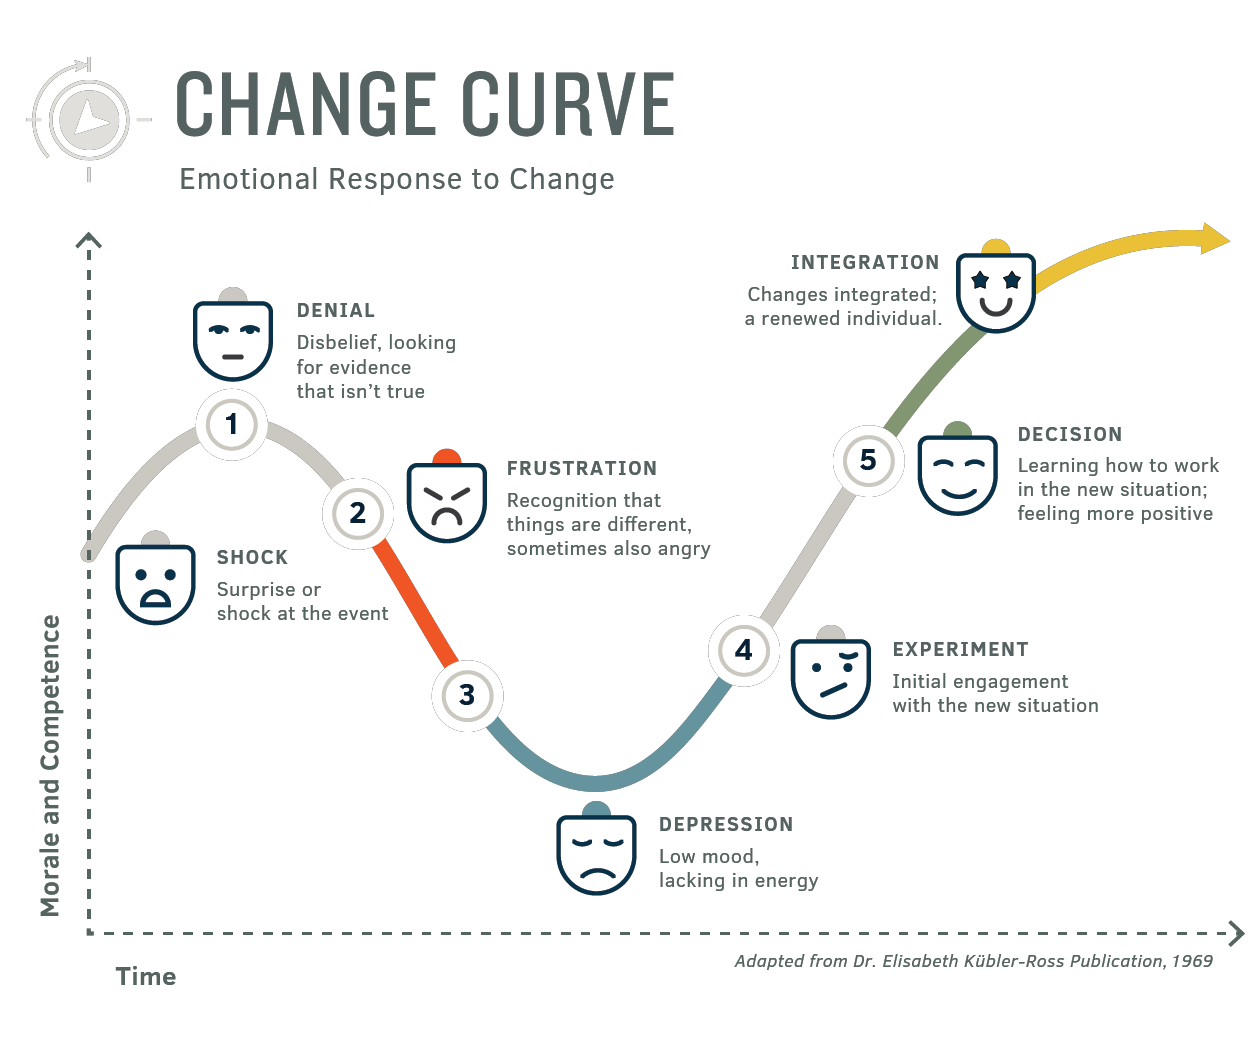
\includegraphics[width=1.0\textwidth]{image.png} 
    \caption{A curve represents the emotional state of a leader throughout time.}
    \label{fig:your-label}
\end{figure}

\subsection{Attempting to Do Everything: A Common Mistake}
Common Mistake: Managers often fall into the trap of attempting to do everything, driven by psychological and professional factors.

\subsection{The Consequences of Overcommitment}
Negative Impacts: Overcommitment leads to compromised decision-making and deteriorating team dynamics, underscoring the need for a resilient leadership approach.


\subsection{The Manager's Superpower: Intentional Task Delegation}
Delegation Strategy: Introduces intentional task delegation as a managerial superpower, empowering team members and fostering sustainability and growth.


\section{Strategic Decision-Making}
In the ever-evolving landscape of engineering management, strategic decision-making is a cornerstone of effective leadership. This section explores the imperative for managers to adapt to new leadership roles, acknowledging that the expansion of responsibilities demands a shift in approach. It underscores the need for a strategic mindset to navigate the challenges and seize
the opportunities that come with elevated leadership positions.

\subsection{Adapting to New Leadership Roles}
Critical Phase: Exploring adjustments needed when stepping into expanded leadership responsibilities, emphasizing personal growth and maintaining effectiveness.

\subsection{Choosing What to Prioritize: The Bad News Test}
Strategic Prioritization: Introduces the "Bad News Test" as a tool for identifying tasks demanding attention, aiding leaders in informed decision-making.

\subsection{Delegating Tasks Safely and Effectively}
Delegation Art: Explores effective task delegation, outlining strategies for identifying suitable tasks, selecting competent team members, and setting clear expectations.


\subsection{Focusing on Critical Priorities}
Pinnacle of Decision-Making: Emphasizes the significance of focusing on critical priorities to align efforts with overarching goals and ensure long-term success.


\section{Transparent Leadership}
Transparent leadership, vital for effective management, is explored in this section. It delves into principles fostering trust, collaboration, and a shared vision within the team, emphasizing its significance in navigating the complexities of engineering management.

\subsection{Communicating Priorities and Changes}
Effective leadership requires transparent communication. This part focuses on articulating priorities and changes clearly, exploring strategies to align the team with evolving goals. Transparent communication is pivotal for creating a cohesive and informed team dynamic.

\subsection{Building Trust Through Open Communication} 
Trust, foundational for strong teams, is built through open communication. The section explores how leaders establish trust by transparently communicating decisions, challenges, and changes. Creating a culture where team members feel valued and informed is central to building trust.

\subsection{Empowering Team Members Through Delegation} 
Empowering team members is a core aspect of transparent leadership. This part highlights delegation as a means of empowerment, emphasizing transparent communication of responsibilities and expectations. Leaders create an environment where team members feel trusted and motivated to contribute.

\subsection{Leveraging Prioritization for Team Growth} 
Effective prioritization benefits not only the manager but also contributes to team growth. The section explores how leaders strategically leverage prioritization to foster team growth, creating opportunities for skill development, collaboration, and professional advancement.

Transparent leadership, encompassing clear communication, trust-building, empowerment through delegation, and strategic prioritization, becomes a powerful framework for nurturing a positive and growth-oriented team culture within the realm of engineering management.


\section{Achieving Success Through Intentional Leadership}
Effective engineering management reaches its pinnacle with intentional leadership. This section explores strategies for success, navigating challenges, fostering growth, and creating a positive impact on teams and the broader organization.

\subsection{Avoiding Secretive Slippages: The Importance of Transparency} 
Transparency is vital for intentional leadership success. This part highlights the drawbacks of secretive practices, emphasizing the need for openness in addressing challenges promptly. By avoiding secrecy, leaders build trust and accountability.

\subsection{Communicating Priorities to Stakeholders} 
Effective communication extends to stakeholders. This section underscores transparently communicating priorities to external parties, outlining methods for aligning the manager’s vision with broader organizational understanding.

\subsection{Saying 'No' to Create Growth Opportunities for Others} 
Strategic decision-making includes saying 'no' with intentionality. It explores how leaders use this to protect their priorities and create growth opportunities for others. Selective task declination opens space for team members to step up.

\subsection{Scaling Leadership and Team Growth} 
Scaling leadership extends impact beyond individual efforts. This part delves into strategies for scaling leadership and fostering team growth. It emphasizes how intentional leadership practices contribute to continuous improvement and overall scalability. Success is viewed not just personally but as collective team growth.

Achieving success through intentional leadership involves openly navigating challenges, effective stakeholder communication, strategic decision-making, and ensuring a positive impact scales leadership and team growth in the dynamic realm of engineering management.


\section{Critical Thinking}
Effective leadership often requires a shift from doing more tasks to strategically leading. This critical thinking section explores key aspects of the "Do Less, Lead More" philosophy, prompting reflection on its implications and potential challenges.

\subsection{Reflections and Analysis}
\begin{itemize}
    \item How does the idea of transitioning from doing more to leading strategically resonate with your current leadership approach? \\
    Consider instances where strategic leadership could have a more significant impact than hands-on involvement.

    \item In what ways have you experienced challenges when trying to do everything as a manager? \\
    Evaluate the benefits of recognizing and openly acknowledging limitations in a leadership role.
    
    \item How comfortable are you with delegating tasks? What factors influence your delegation decisions? \\
    Assess the potential benefits and drawbacks of intentional task delegation within a team.
    
    \item How do you currently prioritize tasks, and what criteria guide your decision-making process? \\
    Explore the impact of narrowing focus on critical tasks and how it aligns with overall team goals.

    
    \item Consider the challenges you foresee in transitioning from a hands-on manager to a strategic leader.\\
    Develop strategies to overcome potential obstacles and ensure a smooth transition.
    
\end{itemize}


\section{Conclusion}
As the discussion on strategic leadership in engineering management concludes, the section reflects on key insights. It provides a comprehensive view of the transition from task management to strategic leadership.

\subsection{Embracing the Intense Growth Cycle}
Embracing the intense growth cycle is vital for leadership evolution. This subsection emphasizes the cyclical nature of growth, encouraging leaders to view challenges and achievements as opportunities for continuous improvement and adaptation.

\subsection{The Path to Becoming a Promoted Leader}
Aspiring leaders discover the path to promotion in this subsection. It explores defining characteristics, strategies, and intentional practices that differentiate leaders. The narrative encourages a proactive approach to personal and team growth, paving the way for elevated positions.

\subsection{Final Thoughts on Strategic Leadership in Engineering Management}
Concluding reflections on strategic leadership encapsulate the essence of the discussed principles. It highlights the significance of intentional decision-making, transparent communication, and empowering team members. This section serves as a takeaway, offering readers a synthesized understanding of effective leadership in the dynamic realm of engineering management.

\newpage

\addcontentsline{toc}{section}{References}

\section*{References\vspace{\baselineskip}}
\begin{enumerate}
    \item Womersley, K. (2023). Do Less, Lead More. In \textit{97 Things Every Engineering Manager Should Know}.
    \item \href{https://d1wqtxts1xzle7.cloudfront.net/44281214/Enhancing_the_Benefits_and_Overcoming_th20160331-30923-1dg1jj9-libre.pdf?1459484708=&response-content-disposition=inline%3B+filename%3DEnhancing_the_Benefits_and_Overcoming_th.pdf&Expires=1701301623&Signature=G6tq5ZEDupVmoRkvGZNQhYYWUDko9Iemqd6uI01oL9ml2Xy2N8i6LscLHJWyM0~Uihi6wuyCCeSQlbn1gy25JtOJGWbWlCwH2U3vDxIGsLntH86JhVZ-kmZxvjSB9UunZUJiC1CKDASrHYIwhPvjEFcgMCDTFOVzwHXu20GCDw3jm1halgrf4CdPW4smBbGv4RsSEGQPE896On4Fq5AooSKW98wrGDHrQPFJDzZH~RhC4~FWGuBMnSfpV9Jblp~c19y5d6kpfF06CxmsxK-gjSxfoGgnoys4BWDgQ-n8nuYk3JVTv6DHi-mkkSrV3QJw1ZNdREHzOknoTLTIPuRwMQ__&Key-Pair-Id=APKAJLOHF5GGSLRBV4ZA}{Enhancing the Benefits and Overcoming the Pitfalls of Goal Setting}
    \item \href{https://books.google.ca/books?hl=en&lr=&id=EGFPDAAAQBAJ&oi=fnd&pg=PA7&dq=Do+Less,+Lead+more&ots=YAZwk04QIC&sig=Y19gqgWCzry_I-GmdG1u3ecUJGs#v=onepage&q&f=false}{The Coaching Habit: Say Less, Ask More and Change the Way You Lead Forever - By Michael Bungay Stanier}
    \item \href{https://journals.aom.org/doi/abs/10.5465/254541}{The Management Theory Jungle}
    \item \href{https://www.jstor.org/stable/43999296}{Overcommitment as a predictor of effort-reward imbalance}
    \item \href{https://www.tandfonline.com/doi/full/10.1080/13683500.2015.1127337}{The manager's dilemma: a conceptualization of online review manipulation strategies}
    \item \href{https://www.sciencedirect.com/science/article/pii/S0167268114001449}{An experimental analysis of transparent leadership}
    \item \href{https://advancesinsocialwork.iupui.edu/index.php/advancesinsocialwork/article/view/18606}{Intentional Leadership Planning and Development}
    \item \href{https://link.springer.com/chapter/10.1007/978-3-319-11107-0_9}{Leading Teams Effectively: Motivating and Prioritizing Work}
    \item \href{https://hypercontext.com/blog/work-goals/engineering-goals}{Engineering goals: How to set goals for high-performing teams - Hypercontext}
    \item \href{https://sponge.io/how-to-lead-a-team-through-disruption-and-change/}{How to Lead a Team through Disruption and Change}
    \item \href{https://ctocraft.com/blog/from-zero-to-cto-katie-womersley-is-in-the-spotlight/}{From Zero to CTO: Katie Womersley is in the spotlight}
    \item \href{https://youtube.com/watch?v=lam-94VHHsM}{Building and scaling distributed teams - Katie Womersley}
    \item \href{https://link.springer.com/article/10.1007/s10551-012-1299-1}{Leader Ethical Decision-Making in Organizations}
    \item \href{https://chat.openai.com/}{OpenAI. (2023). ChatGPT v3.5 [Large language model]. https://chat.openai.com/}
    \item \href{https://dokumen.pub/97-things-every-engineering-manager-should-know-collective-wisdom-from-the-experts-1nbsped-1492050903-9781492050902.html}{97 Things Every Engineering Manager Should Know: Collective Wisdom from the Experts}
    \item \href{https://www.managersclub.com/katie-womersley/}{Interview with Katie Womersley, Director of Engineering at Buffer}
    \item \href{https://gmdconsulting.eu/nykerk/wp-content/uploads/2020/02/On_Becoming_a_Leader-Bennis-summary.pdf}{"On becoming a Leader" - Warren Bennis}

\end{enumerate}


\end{document}
